\section{Stromrichterschaltung}
\subsection{Gruppierung}
\subsubsection{nach Steuerung}
\begin{itemize}
    \item Ungesteuerte Stromrichter:
        \subitem Das Verhältniss von Eingans- zu Ausgangsspannung wird durch die Stromrichterschaltung festzgesetzt
    \item Gesteuerte Stromrichter
        \subitem Das Verhältniss von Eingans- zu Ausgangsspannung wird durch Steuereingriff am Halbleiterschalter verändert. 
\end{itemize}

\subsubsection{nach Führung}
\href{https://de.wikipedia.org/wiki/Kommutierung}{Kommuntierung WIKI}\newline
\begin{minipage}{0.6\linewidth}
Bzw nach der Herlkunft der Kommutierungsspannung.\newline
Kommutierung bedeutet die Wechslung des Stromflusses von einem HL-Ventil auf ein anderes.
\begin{itemize}
    \item Netzgeführte Schaltung
        \subitem Kommutierungsspannung vom Netzwerk
    \item Lastgeführte Schaltung
        \subitem Kommuntierungsspannung wird durch Lastkreis (zb Synchronmotor) gesteuert
    \item Selbstgeführte Schalung
        \subitem Kommutierungsspannung wird selbst erzeugt
\end{itemize}
\end{minipage}
\begin{minipage}{0.4\linewidth}
    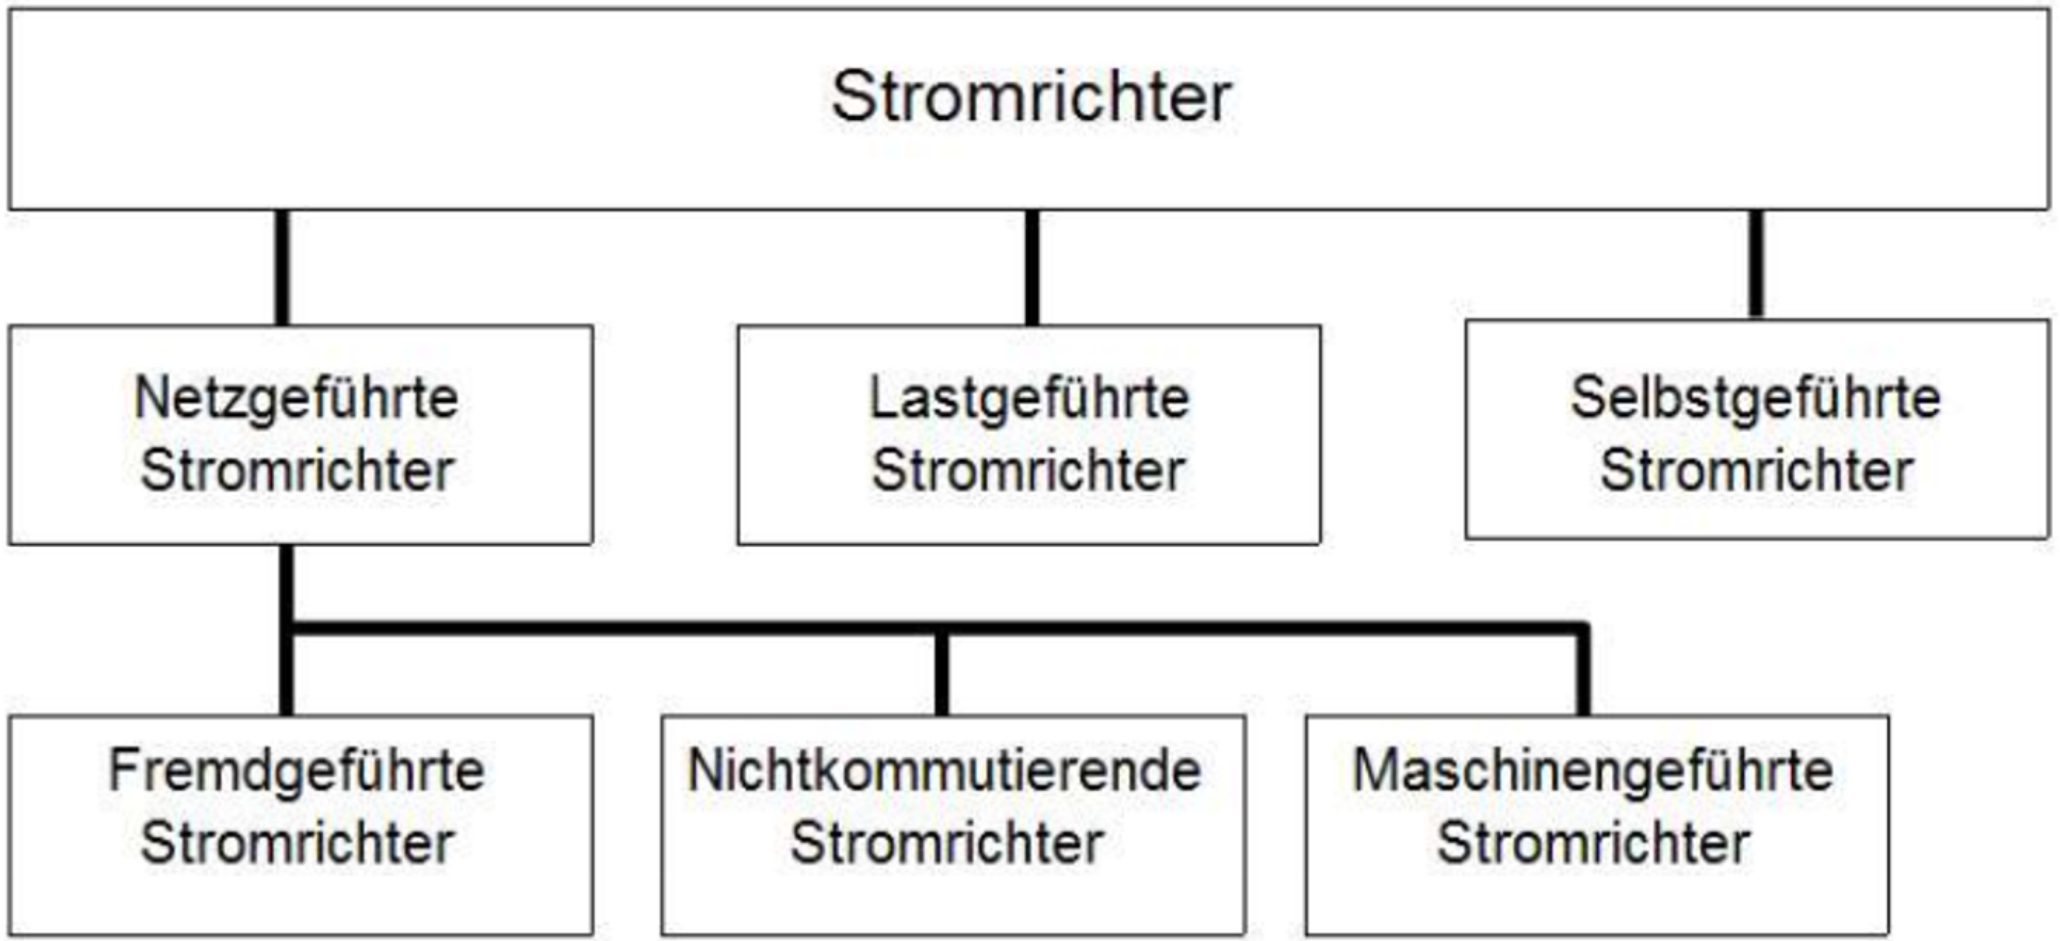
\includegraphics[width=\linewidth]{images/StromrichterKennzeichnung}\newline
\end{minipage}

\subsection{Kennzeichnung}
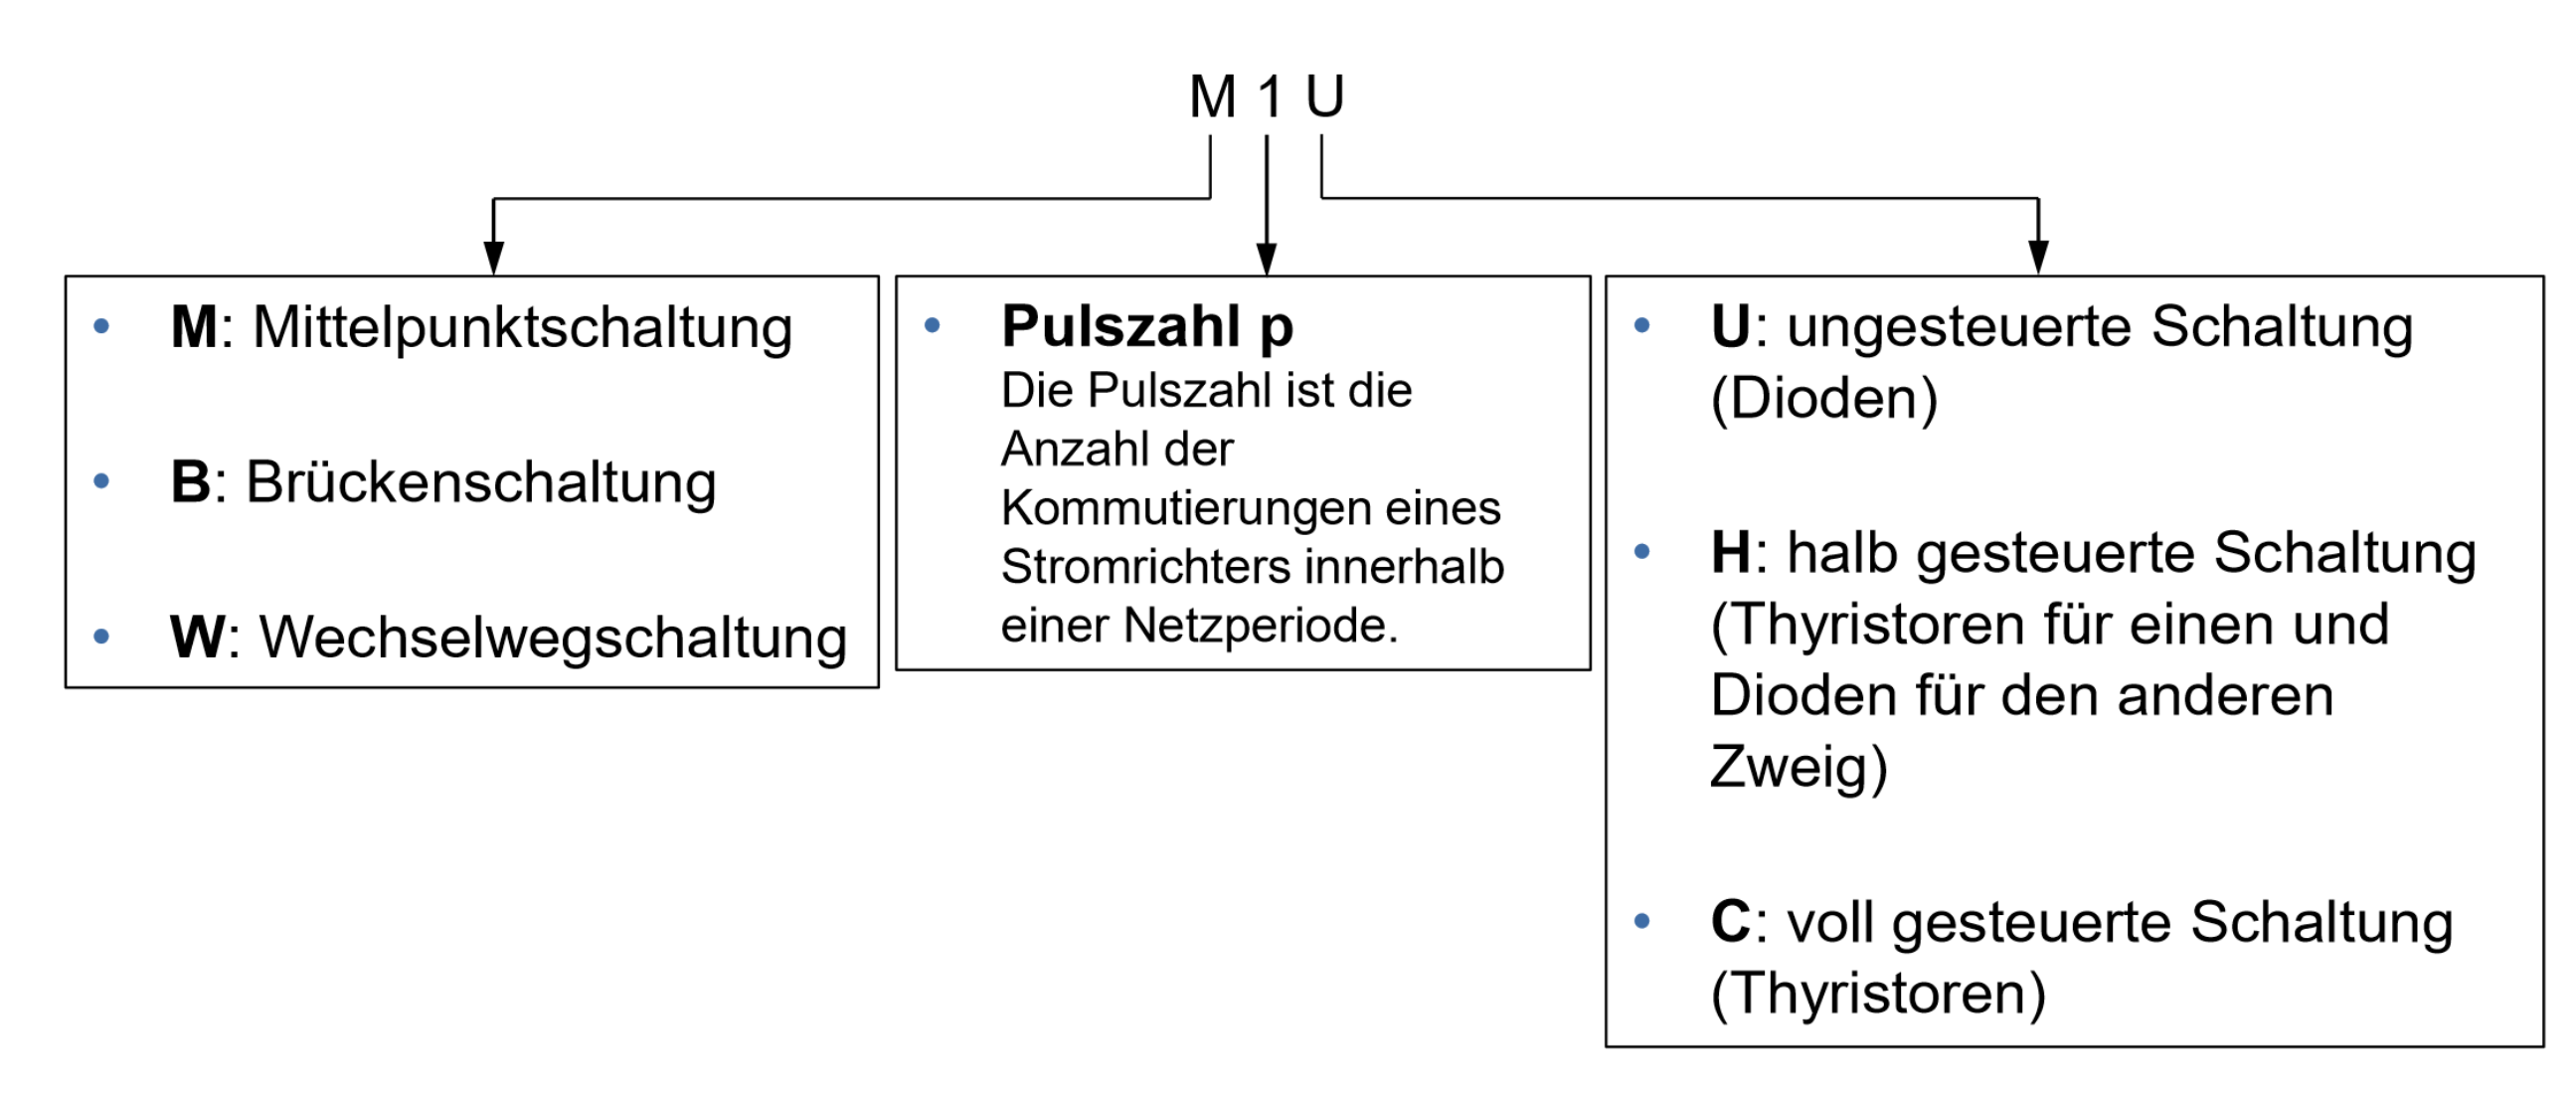
\includegraphics[width=0.9\linewidth]{images/SRKennzeichnung}\newline
\href{https://de.wikipedia.org/wiki/Gleichrichter}{Gleichrichter WIKI}

%===================================================================
\clearpage